%\cajita{Créditos otorgados a la pequeña y mediana empresa por sexo, según rama de actividad económica}{Según los Registros de la Unidad Financiera Programa Nacional para el Desarrollo de la MIPYME del Ministerio de Economía, las principales actividades económicas a las que se entregaron créditos a mujeres en 2022 fueron a Comercio con 640 créditos, seguido de Servicios con 91 créditos y Artesanías con 9 créditos. En 2018 se entregaron 865 créditos en Comercio, seguido de Servicios con 87 créditos e Industria con 31 créditos otorgados a mujeres. }{Créditos otorgados a la pequeña y mediana empresa por sexo, según rama de actividad económica (2018 y 2022) (número de créditos)}{República de Guatemala, Instituto Nacional de Estadística}{\begin{tabular}[t]{ccccc}
\toprule
\multicolumn{1}{c}{\textbf{ }} & \multicolumn{2}{c}{\textbf{2018}} & \multicolumn{2}{c}{\textbf{2022}} \\
\cmidrule(l{3pt}r{3pt}){2-3} \cmidrule(l{3pt}r{3pt}){4-5}
\textbf{Actividad Económica} & \textbf{Mujeres} & \textbf{Hombres} & \textbf{Mujeres} & \textbf{Hombres}\\
\midrule
\cellcolor[HTML]{B6B3FF}{Comercio} & \cellcolor[HTML]{B6B3FF}{865} & \cellcolor[HTML]{B6B3FF}{1050} & \cellcolor[HTML]{B6B3FF}{640} & \cellcolor[HTML]{B6B3FF}{836}\\
Servicios & 87 & 155 & 91 & 159\\
\cellcolor[HTML]{B6B3FF}{Industria} & \cellcolor[HTML]{B6B3FF}{31} & \cellcolor[HTML]{B6B3FF}{52} & \cellcolor[HTML]{B6B3FF}{9} & \cellcolor[HTML]{B6B3FF}{30}\\
Artesanía & 12 & 26 & 15 & 18\\
\cellcolor[HTML]{B6B3FF}{Agroindustria} & \cellcolor[HTML]{B6B3FF}{5} & \cellcolor[HTML]{B6B3FF}{5} & \cellcolor[HTML]{B6B3FF}{11} & \cellcolor[HTML]{B6B3FF}{14}\\
\bottomrule
\end{tabular}
}{Registros Unidad Financiera Programa Nacional para el Desarrollo de la MIPYME, MINECO 2023}{}

%\cajita{Proporción de tiempo dedicado a quehaceres domésticos y cuidados no remunerados por grupos de edad}{La proporción del día que las mujeres dedican a realizar quehaceres domésticos y de cuidado no remunerado es de 20.6\% en las mujeres de 15 a 29 años, seguido de 25.1\% en las mujeres de 30 a 65 años y  de 2.9\% en las mujeres mayores a 65 años. }{Proporción de tiempo dedicado a quehaceres domésticos y de cuidados no remunerados por grupos de edad (porcentaje)}{República de Guatemala, Instituto Nacional de Estadística} {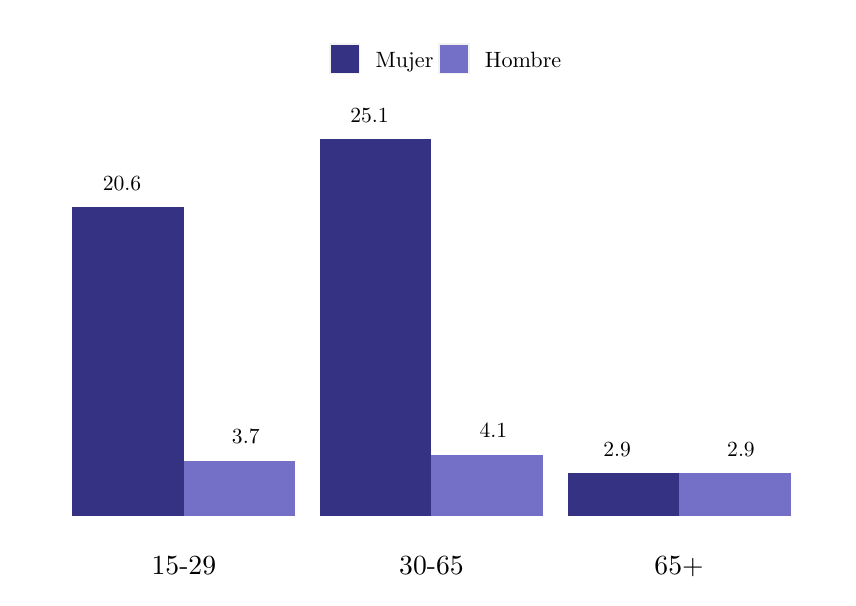
\begin{tikzpicture}[x=1pt,y=1pt]% Created by tikzDevice version 0.12.4 on 2023-05-05 11:16:49
% !TEX encoding = UTF-8 Unicode
\definecolor{fillColor}{RGB}{255,255,255}
\path[use as bounding box,fill=fillColor,fill opacity=0.00] (0,0) rectangle (289.08,198.74);
\begin{scope}
\path[clip] (  0.00,  0.00) rectangle (289.08,198.74);

\path[] (  0.00,  0.00) rectangle (289.08,198.74);
\end{scope}
\begin{scope}
\path[clip] (  0.00,  0.00) rectangle (289.08,198.74);
\definecolor{fillColor}{RGB}{54,50,131}

\path[fill=fillColor] ( 16.17, 22.21) rectangle ( 56.44,133.79);

\path[fill=fillColor] (105.65, 22.21) rectangle (145.91,158.54);

\path[fill=fillColor] (195.13, 22.21) rectangle (235.39, 37.71);
\definecolor{fillColor}{RGB}{116,112,200}

\path[fill=fillColor] ( 56.44, 22.21) rectangle ( 96.70, 42.27);

\path[fill=fillColor] (145.91, 22.21) rectangle (186.18, 44.46);

\path[fill=fillColor] (235.39, 22.21) rectangle (275.66, 37.71);
\definecolor{drawColor}{RGB}{0,0,0}

\node[text=drawColor,anchor=base,inner sep=0pt, outer sep=0pt, scale=  0.78] at ( 34.07,139.86) {20.6};

\node[text=drawColor,anchor=base,inner sep=0pt, outer sep=0pt, scale=  0.78] at (123.55,164.61) {25.1};

\node[text=drawColor,anchor=base,inner sep=0pt, outer sep=0pt, scale=  0.78] at (213.02, 43.77) {2.9};

\node[text=drawColor,anchor=base,inner sep=0pt, outer sep=0pt, scale=  0.78] at ( 78.81, 48.34) {3.7};

\node[text=drawColor,anchor=base,inner sep=0pt, outer sep=0pt, scale=  0.78] at (168.28, 50.52) {4.1};

\node[text=drawColor,anchor=base,inner sep=0pt, outer sep=0pt, scale=  0.78] at (257.76, 43.77) {2.9};

\path[] (  2.75, 22.21) --
	(289.08, 22.21);

\path[] (  2.75, 49.33) --
	(289.08, 49.33);

\path[] (  2.75, 76.44) --
	(289.08, 76.44);

\path[] (  2.75,103.55) --
	(289.08,103.55);

\path[] (  2.75,130.66) --
	(289.08,130.66);

\path[] (  2.75,157.77) --
	(289.08,157.77);

\path[] (  2.75, 15.40) rectangle (289.08,165.36);
\end{scope}
\begin{scope}
\path[clip] (  0.00,  0.00) rectangle (289.08,198.74);

\path[] (  2.75, 15.40) --
	(  2.75,165.36);
\end{scope}
\begin{scope}
\path[clip] (  0.00,  0.00) rectangle (289.08,198.74);

\path[] (  0.00, 22.21) --
	(  2.75, 22.21);

\path[] (  0.00, 49.33) --
	(  2.75, 49.33);

\path[] (  0.00, 76.44) --
	(  2.75, 76.44);

\path[] (  0.00,103.55) --
	(  2.75,103.55);

\path[] (  0.00,130.66) --
	(  2.75,130.66);

\path[] (  0.00,157.77) --
	(  2.75,157.77);
\end{scope}
\begin{scope}
\path[clip] (  0.00,  0.00) rectangle (289.08,198.74);

\path[] (  2.75, 15.40) --
	(289.08, 15.40);
\end{scope}
\begin{scope}
\path[clip] (  0.00,  0.00) rectangle (289.08,198.74);

\path[] ( 56.44, 12.65) --
	( 56.44, 15.40);

\path[] (145.91, 12.65) --
	(145.91, 15.40);

\path[] (235.39, 12.65) --
	(235.39, 15.40);
\end{scope}
\begin{scope}
\path[clip] (  0.00,  0.00) rectangle (289.08,198.74);
\definecolor{drawColor}{RGB}{0,0,0}

\node[text=drawColor,anchor=base,inner sep=0pt, outer sep=0pt, scale=  1.00] at ( 56.44,  1.32) {15-29};

\node[text=drawColor,anchor=base,inner sep=0pt, outer sep=0pt, scale=  1.00] at (145.91,  1.32) {30-65};

\node[text=drawColor,anchor=base,inner sep=0pt, outer sep=0pt, scale=  1.00] at (235.39,  1.32) {65+};
\end{scope}
\begin{scope}
\path[clip] (  0.00,  0.00) rectangle (289.08,198.74);
\definecolor{fillColor}{RGB}{255,255,255}

\path[fill=fillColor] ( 97.83,176.36) rectangle (194.00,198.74);
\end{scope}
\begin{scope}
\path[clip] (  0.00,  0.00) rectangle (289.08,198.74);
\definecolor{fillColor}{gray}{0.95}

\path[fill=fillColor] (108.83,181.86) rectangle (120.21,193.24);
\end{scope}
\begin{scope}
\path[clip] (  0.00,  0.00) rectangle (289.08,198.74);
\definecolor{fillColor}{RGB}{54,50,131}

\path[fill=fillColor] (109.49,182.52) rectangle (119.55,192.58);
\end{scope}
\begin{scope}
\path[clip] (  0.00,  0.00) rectangle (289.08,198.74);
\definecolor{fillColor}{gray}{0.95}

\path[fill=fillColor] (148.37,181.86) rectangle (159.75,193.24);
\end{scope}
\begin{scope}
\path[clip] (  0.00,  0.00) rectangle (289.08,198.74);
\definecolor{fillColor}{RGB}{116,112,200}

\path[fill=fillColor] (149.04,182.52) rectangle (159.09,192.58);
\end{scope}
\begin{scope}
\path[clip] (  0.00,  0.00) rectangle (289.08,198.74);
\definecolor{drawColor}{RGB}{0,0,0}

\node[text=drawColor,anchor=base west,inner sep=0pt, outer sep=0pt, scale=  0.80] at (125.71,184.43) {Mujer};
\end{scope}
\begin{scope}
\path[clip] (  0.00,  0.00) rectangle (289.08,198.74);
\definecolor{drawColor}{RGB}{0,0,0}

\node[text=drawColor,anchor=base west,inner sep=0pt, outer sep=0pt, scale=  0.80] at (165.25,184.43) {Hombre};
\end{scope}
\end{tikzpicture}}{INE - ENEI 2022}{}

%\cajota{Población por sexo, según grupos de edad}{El sector informal guatemalteco comprende a la Población Ocupada (PO) que labora como empleadores, empleados y obreros de empresas con menos de 6 personas, trabajadores por cuenta propia o autónoma (excluyendo profesionales y técnicos), familiares no remunerados de los empleadores o personas ocupadas en servicio doméstico. Su contraparte, el sector formal, está comprendido por la población ocupada que no está en el sector informal. 

En el año 2022 las mujeres integraron el 27.9\% del sector informal y el 9.2\% del sector formal. }{Población por sexo, según grupos de edad}{República de Guatemala, Instituto Nacional de Estadística, en miles de personas}{\begin{tikzpicture}[x=1pt,y=1pt, scale=1.75]% Created by tikzDevice version 0.12.4 on 2023-05-04 15:41:55
% !TEX encoding = UTF-8 Unicode
\definecolor{fillColor}{RGB}{255,255,255}
\path[use as bounding box,fill=fillColor,fill opacity=0.00] (0,0) rectangle (289.08,198.74);
\begin{scope}
\path[clip] (  0.00,  0.00) rectangle (289.08,198.74);

\path[] (  0.00,  0.00) rectangle (289.08,198.74);
\end{scope}
\begin{scope}
\path[clip] (  0.00,  0.00) rectangle (289.08,198.74);
\definecolor{fillColor}{RGB}{54,50,131}

\path[fill=fillColor] ( 23.00, 21.09) rectangle ( 75.55, 52.92);

\path[fill=fillColor] (154.39, 21.09) rectangle (206.95,117.47);
\definecolor{fillColor}{RGB}{116,112,200}

\path[fill=fillColor] ( 82.13, 21.09) rectangle (134.68, 89.08);

\path[fill=fillColor] (213.53, 21.09) rectangle (266.08,170.58);
\definecolor{drawColor}{RGB}{0,0,0}

\path[draw=drawColor,line width= 0.6pt,line join=round] (-289.08, 21.09) -- (578.16, 21.09);

\node[text=drawColor,anchor=base,inner sep=0pt, outer sep=0pt, scale=  0.83] at ( 49.27, 56.15) {9.2};

\node[text=drawColor,anchor=base,inner sep=0pt, outer sep=0pt, scale=  0.83] at (180.68,120.70) {27.9};

\node[text=drawColor,anchor=base,inner sep=0pt, outer sep=0pt, scale=  0.83] at (108.41, 92.31) {19.7};

\node[text=drawColor,anchor=base,inner sep=0pt, outer sep=0pt, scale=  0.83] at (239.81,173.81) {43.2};

\path[] (  0.00, 21.09) rectangle (289.08,170.58);

\path[] ( 78.84, 21.09) --
	( 78.84,170.58);

\path[] (210.24, 21.09) --
	(210.24,170.58);

\path[] (  0.00, 21.09) rectangle (289.08,170.58);
\end{scope}
\begin{scope}
\path[clip] (  0.00,  0.00) rectangle (289.08,198.74);

\path[] (  0.00, 21.09) --
	(  0.00,170.58);
\end{scope}
\begin{scope}
\path[clip] (  0.00,  0.00) rectangle (289.08,198.74);

\path[] (  0.00, 21.09) --
	(289.08, 21.09);
\end{scope}
\begin{scope}
\path[clip] (  0.00,  0.00) rectangle (289.08,198.74);

\path[] ( 78.84, 18.34) --
	( 78.84, 21.09);

\path[] (210.24, 18.34) --
	(210.24, 21.09);
\end{scope}
\begin{scope}
\path[clip] (  0.00,  0.00) rectangle (289.08,198.74);
\definecolor{drawColor}{RGB}{0,0,0}

\node[text=drawColor,anchor=base,inner sep=0pt, outer sep=0pt, scale=  1.00] at ( 78.84,  7.01) {Formal};

\node[text=drawColor,anchor=base,inner sep=0pt, outer sep=0pt, scale=  1.00] at (210.24,  7.01) {infromal};
\end{scope}
\begin{scope}
\path[clip] (  0.00,  0.00) rectangle (289.08,198.74);
\coordinate (apoyo) at (59.42,189.21);
\coordinate (longitudFicticia) at (7.11,9.53);
\coordinate (longitud) at (7.11,7.11);
\coordinate (desX) at (135.34,0);
\coordinate (desY) at (0,1.21);
\definecolor[named]{ct1}{HTML}{
363283
}
\definecolor[named]{ct2}{HTML}{
7470C8
}
\definecolor[named]{ctb1}{HTML}{
363283
}
\definecolor[named]{ctb2}{HTML}{
7470C8
}
\path [fill=none] (apoyo) rectangle ($(apoyo)+(longitudFicticia)$)
node [xshift=0.3cm,inner sep=0pt, outer sep=0pt,midway,right,scale = 0.9]{Mujer};
\draw [color = ctb1,fill=ct1] ( $(apoyo)  + (desY) $) rectangle ($(apoyo)+ (desY) +(longitud)$);
\path [fill=none] ($(apoyo)+(desX)$) rectangle ($(apoyo)+(desX)+(longitudFicticia)$)
node [xshift=0.3cm,inner sep=0pt, outer sep=0pt,midway,right,scale = 0.9]{Hombre};
\draw [color = ctb2 ,fill=ct2] ( $(apoyo)  + (desY) + (desX) $) rectangle ($(apoyo)+ (desY)+ (desX) +(longitud)$);
\end{scope}
\end{tikzpicture}}{INE - Censo 2018}